% This is a special document class, provided in the file VRARWorkshop.cls
% It contains special format options for the workshop proceedings.
% In this sample document, we illustrate the template's usage.
% It is assumed, that the reader has basic knowledge about the LaTeX System.

% First of all choose the right document class. The default layout style will
% choose English as default language. If you are writing your text in German
% please enable the <german> option here. If you choose English as your
% language, leave out the <german> option. If the option is set, native
% language encoding will be activated i.e. you will be able to type ü
% instead of "u or \"u.
% NOTE: If you are experiencing strange errors when TeXing your document after
% a change to the <german> option, try rebuilding the whole document including
% the bibTeX file.



% German option set
%\documentclass[german]{VRARWorkshop}
% English option set
\documentclass{VRARWorkshop}

\usepackage[utf8]{inputenc}
\usepackage[T1]{fontenc}
\usepackage{ngerman}
\usepackage[hidelinks]{hyperref}
% Define your paper's title. This has to be done BEFORE \begin{document}!
\title{Visual Raytrace: An Immersive Learning Application}

% Define the list of authors of your paper. This has to be done BEFORE
% \begin{document}!
% one or several authors from the SAME INSTITUTION
%\authors{~}
\authors{Manfred Brill, Benedict S"arota}
% several authors from DIFFERENT INSTITUTIONS
% \authors{Vorname1 Name1\VRARafftag{\ast}, Vorname2 Name2 \VRARafftag{\dagger}}

% Define the list of authors' affiliations. If you have authors from several
% institutions, please choose the table format given below. The class file
% provides the command \VRARafftag{<tagchar>}, which should be used to create
% tags on different institutions.  In order to use it, insert the tag command
% with the corresponding tag character after the author's name and in front of
% the first entry in the affiliation table entry. As tag chars we use \ast,
% \dagger, \star, \ddagger, \diamond, in this order. If you need to include
% more than 5 institutions (which should be highly unlikely) feel free to add
% symbols as appropriate. This also has to be done BEFORE \begin{document}.

% one or several authors from the SAME INSTITUTION
%\affiliations{~} %<---- anonymous submission
\affiliations{
    University of Applied Sciences Kaiserslautern \\
    Amerikastr. 1 \\
    66482 Zweibrücken \\
    Tel.: +49 (0)631 / 37 24 - [5382, 5321] \\
%    Fax: +49 (0)815 / 40 90 - 115 \\
    E-Mail: [manfred.brill, benedict.saerota]@hs-kl.de
}

% several authors from DIFFERENT INSTITUTIONS
%\affiliations{
%\begin{tabular}{cc}
%\VRARafftag{\ast} Musterinstitut1 & \VRARafftag{\dagger} Musterinstitut2\\
%Musterstr. 1  & Musterstr. 1  \\
%08150 Musterstadt & 08150 Musterstadt\\
%Tel.: +49 (0)815 / 40 90 - 158  &  \\
%Fax: +49 (0)815 / 40 90 - 115 & \\
%E-Mail: mustermann@provider.de &
%\end{tabular}
%}

% Write up your abstract here...
\abstract{%
Visual Raytrace is an immersive learning application supporting students in a computer graphics class to create
their own version of a working raytracing software.
the users can interact with all ingredients of a raytracer like camera model, framebuffer, scene description,
sampling, reflections models or texture mapping.
}

% Give some keywords
\keywords{Virtual Reality, Education, Immersive Learning, Computer Graphics Classes, Raytraing}

\graphicspath{{figures/}} % Location of the graphics files

\usepackage[figurename=Figure]{caption}
\renewcommand{\refname}{References}
% Finally you get to work ;-) Start your document and...
\begin{document}
% ...begin with the introduction section right away. The title format
% will be generated automatically at the top of the page.

\section{Introduction}
Raytracing, introduced by Turner Whitted \cite{whitted_80}, is one of the major topics in
computer graphics classes.
In figure \ref{intro:whitted} we find on of the famous pictures rendered by Whitted.

\begin{figure}[h!]
    \begin{center}
        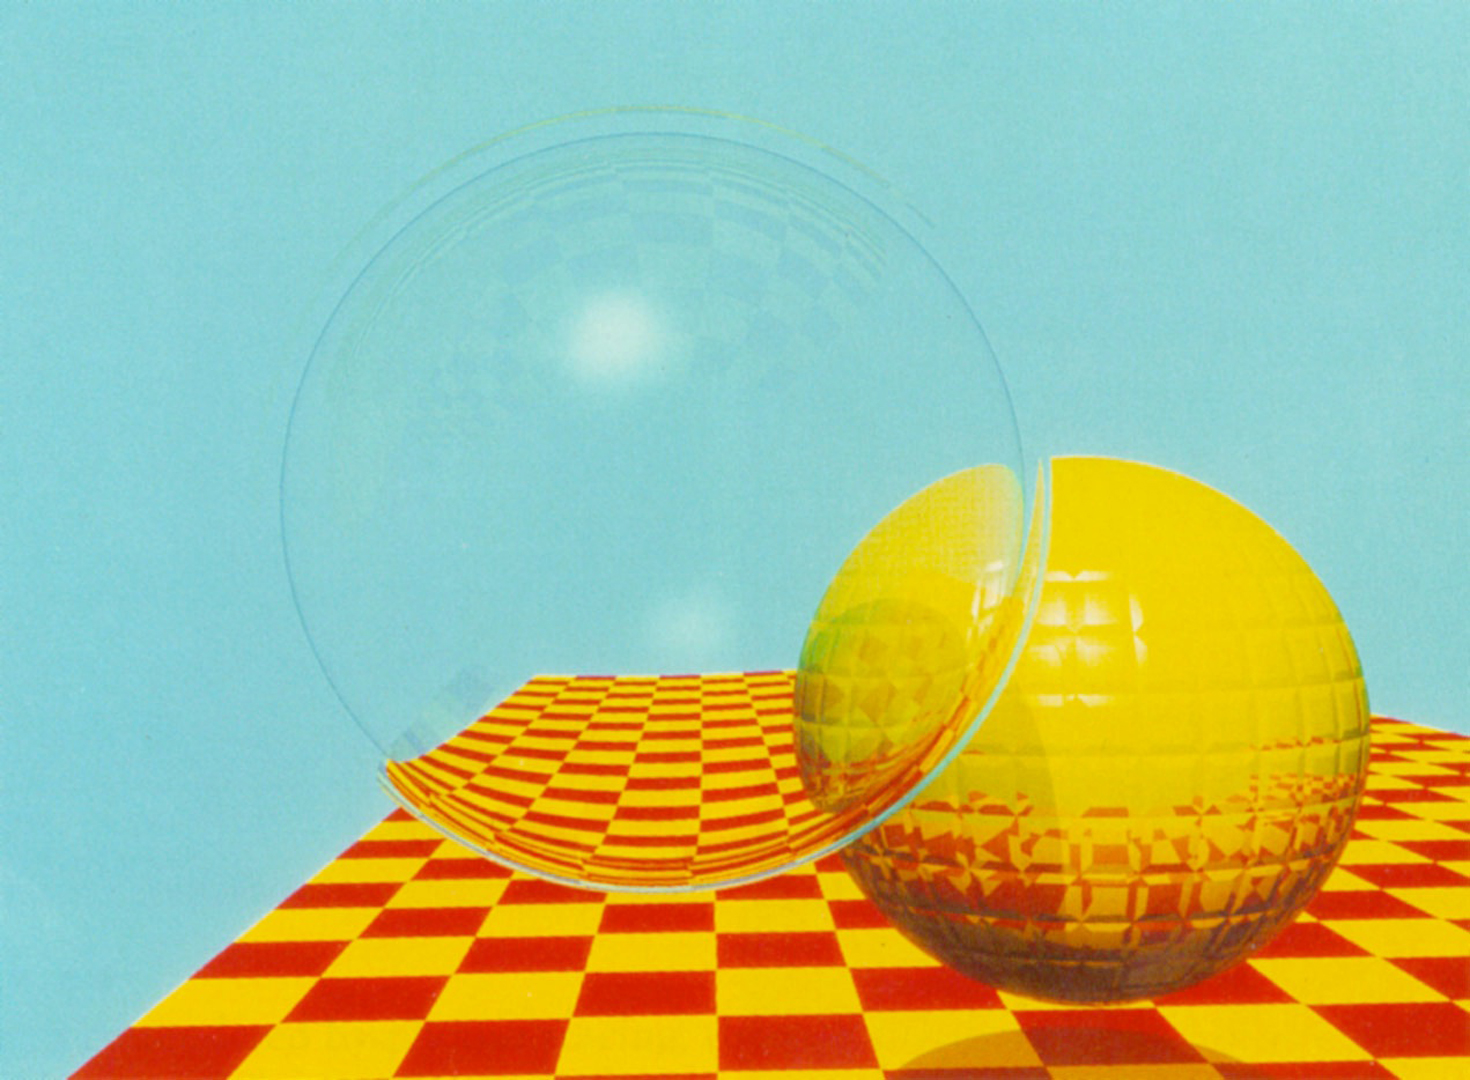
\includegraphics[width=0.35\textwidth]{whitted02.jpg}
        \caption{\label{intro:whitted} Image rendered by Turner Whitted (Source:
        \url{https://de.wikipedia.org/wiki/Datei:Spheres_and_Checkerboard_-_Turner_Whitted.jpg})}
    \end{center}
\end{figure}
Usually students in a computer graphics class implement their version of such a renderer,
after getting the theory in the class.
To achieve this they need to understand the basic concepts of computer graphics like coordinate systems,
cameras, reflection models or texture mapping. To implement a raytracer or another 3D application the students have to
develop a strong visual-spatial ability. Virtual reality applications provide joy of use and support the transfer
from 3D space to a programming language and deepen the understanding of the basic concepts of a raytracer.
%
\section{Visual Raytrace}
We implemented the immersive learning application \textbf{Visual Raytrace} \cite{saerota_21b, visualraytrace} using the Unity Game Engine
and HTC vive Input Utility (\cite{viveInput}). Figure \ref{vray:scene} shows the main features of the application.

\begin{figure}[h!]
    \begin{center}
        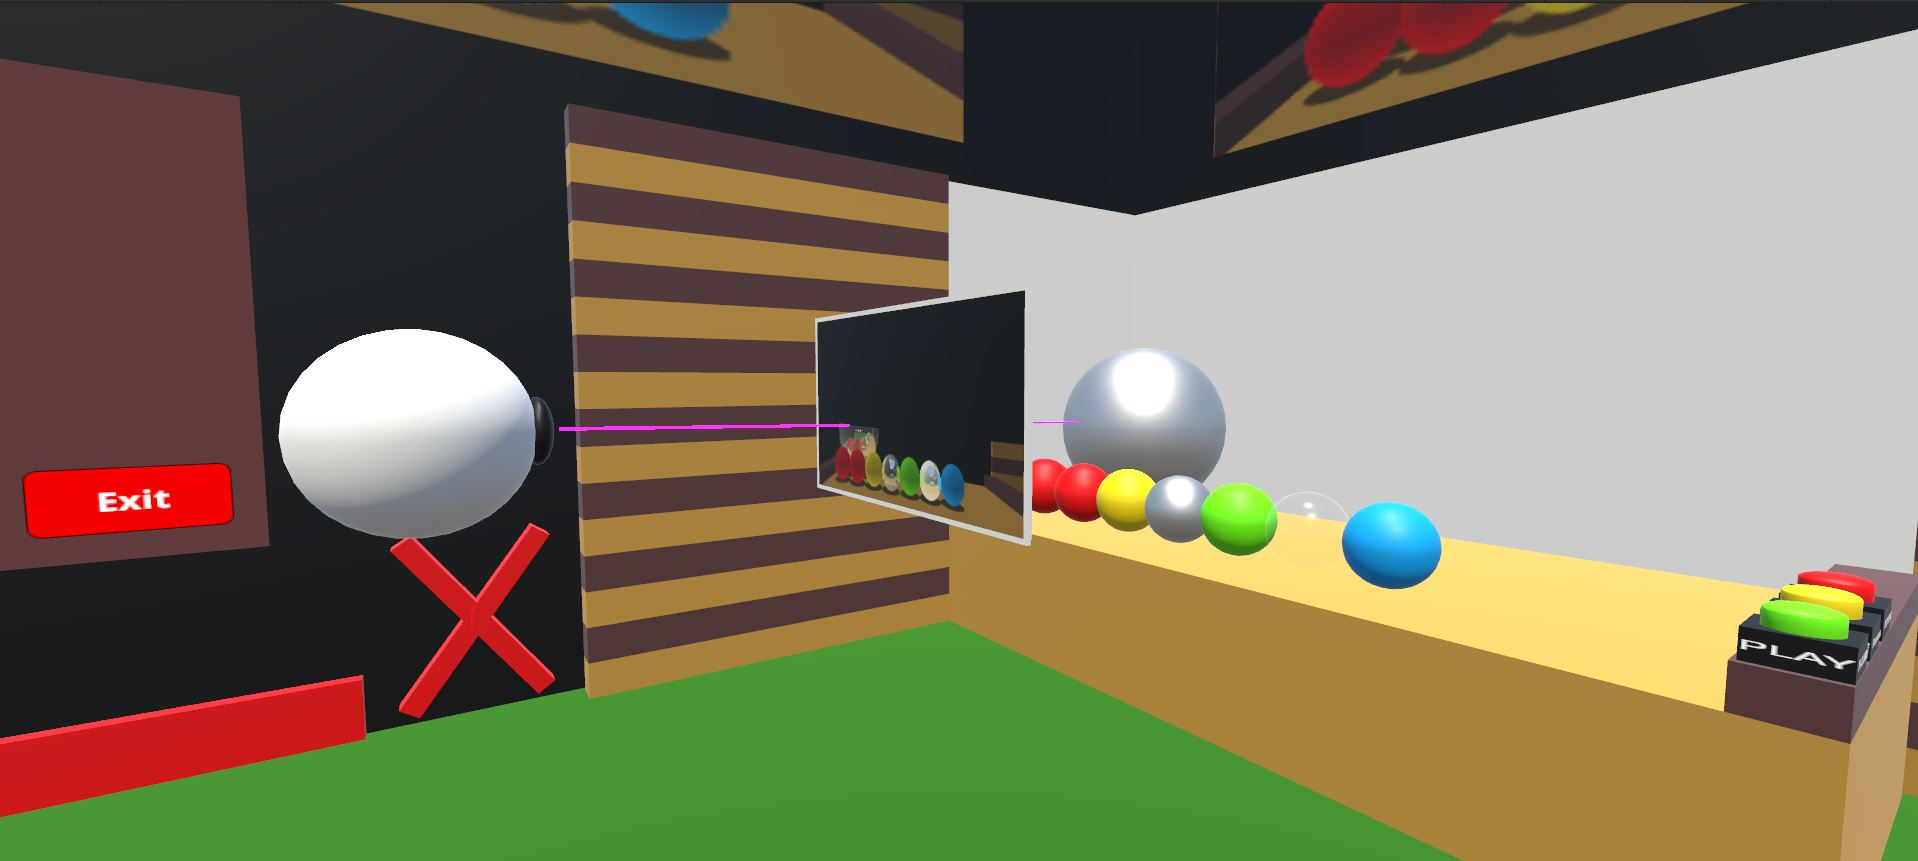
\includegraphics[width=0.55\textwidth]{duringProcess}
        \caption{\label{vray:scene} The elements of a raytracer in an immersive environment}
    \end{center}
\end{figure}
The raytracer is implemented in C\# und is slowed down to make sure the users can follow the path
of the ray and the reflections in the scene until the color of the pixel is finally computed.
The raytracing process can be paused or soptted to get an understanding of the rendering algorithm.
At the end the computed image can be saved for further investigation.

\begin{figure}[h!]
    \begin{center}
        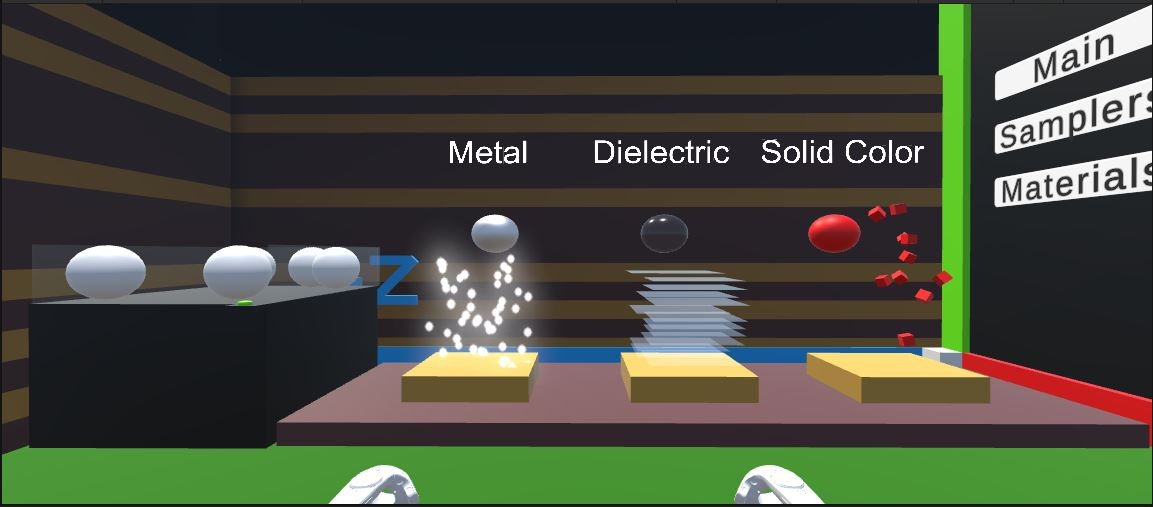
\includegraphics[width=0.55\textwidth]{sphereCreating}
        \caption{\label{vray:materials} Geometric objects and reflection functions for scene definition}
    \end{center}
\end{figure}
The scene can either be defined in VR or can be read from a scene description file. 
Figure \ref{vray:materials} shows the interface for the interactive scene definition.
New objects can be picked and one of the reflection models can be assigned.
Afterwards users position this new object in the rendered scene.
The options for the raytracer can also be set in the immersive environment.
%
\section{Future Work}
We plan to use the immersive learning application in the next computer graphics class in the summer term 2022.
The implementation of a working raytracer is the assignment in the class, so we will
transfer the C\# code for the raytracer to an own repository and link the renderer as a dynamic library.
Another possibility would be to change the programming language used in the computer graphics class
to C\#.  Doing this the learning application and the raytrace could be made both public.
the assignment could then be changed.
This has to be discussed and decided with the lecturers for the next summer term.

It is planned
to implement a change of scenes so the users can dive into the 3D world currently being raytraced
and back..
This way the students can walk around in the scene currently rendered and have a close look to intersection points,
reflections or refractions.

Due to the pandemic situation on our campus we could not evaluate the application with students.
Hopefully we will be able to do this in the winter term 2021/22 at our campus. the results of this
evaluation will help us to improve the usability and joy of use of the application.
Now the software runs in our lab with a HTC Vive Pro and Vive Focus Plus head-mounted displays.
The vive Input Utility supports builds for Google Cardboard or Oculus Android. We also work
on an OpenXR- and WebXR-based versions to support as many platform as possible
to distribute the application on the home equipment of the students.

%set appropriate bib style
\VRARsetbibstyle
\bibliography{sample}

\end{document}
